\documentclass[border=8pt]{standalone}
\usepackage{tikz}
\usetikzlibrary{quantikz2,positioning,arrows.meta,calc,shapes.geometric,decorations.pathreplacing}
\usepackage{mathpazo}
\usepackage{amsmath,amssymb,braket}
\definecolor{qxblue}{HTML}{156082}
\definecolor{qxink}{HTML}{0B1A22}
\definecolor{qxtint}{HTML}{E4EEF3}
\definecolor{qxsand}{HTML}{F5ECD7}
\definecolor{qxrose}{HTML}{F6DEDE}
\definecolor{qxsage}{HTML}{E2EFE3}
\tikzset{g/.style={fill=qxtint,draw=qxink}, o/.style={fill=qxsand,draw=qxink}, e/.style={fill=qxrose,draw=qxink},
  q/.style={fill=qxsage,draw=qxink},
  grp/.style={dashed,rounded corners,draw=qxblue!80,inner xsep=4pt},
  box/.style={draw=qxink,rounded corners=3pt,fill=qxtint,align=center,inner sep=6pt,font=\small},
  arr/.style={-{Stealth[length=2.2mm]},thick,draw=qxink}}
\begin{document}
\begin{tabular}{c}
\begin{quantikz}[row sep=0.4cm, column sep=0.4cm]
\lstick{$\ket{0}^{\otimes n}$} & \qwbundle{n} & \gate[style=g]{H^{\otimes n}} & \gate[style=o]{O_m}\gategroup[1,steps=2,style=grp]{\small Grover iteration $G=D\,O_m$, $\ k\approx\frac{\pi}{4}\sqrt{N}$ times} & \gate[style=g]{D} & \meter{} & \setwiretype{c} \rstick{$m$}
\end{quantikz}\\[8pt]
\begin{tikzpicture}[baseline=(D.base)]\node (D) {$D\;=$};\end{tikzpicture}
\begin{quantikz}[row sep=0.25cm, column sep=0.28cm]
& \gate[style=g]{H} & \gate[style=g]{X} & \ctrl{2} & \gate[style=g]{X} & \gate[style=g]{H} & \\
& \gate[style=g]{H} & \gate[style=g]{X} & \control{} & \gate[style=g]{X} & \gate[style=g]{H} & \\
& \gate[style=g]{H} & \gate[style=g]{X} & \control{} & \gate[style=g]{X} & \gate[style=g]{H} &
\end{quantikz}
\hspace{1.2em}
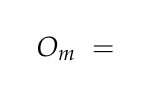
\begin{tikzpicture}[baseline=(O.base)]\node (O) {$O_m\;=$};\end{tikzpicture}
\begin{quantikz}[row sep=0.25cm, column sep=0.28cm]
& \gate[style=g]{X^{\bar m_2}} & \ctrl{2} & \gate[style=g]{X^{\bar m_2}} & \\
& \gate[style=g]{X^{\bar m_1}} & \control{} & \gate[style=g]{X^{\bar m_1}} & \\
& \gate[style=g]{X^{\bar m_0}} & \control{} & \gate[style=g]{X^{\bar m_0}} &
\end{quantikz}
\end{tabular}

\end{document}
